\documentclass{standalone}
  \usepackage{pgfplots}
  \usepackage{amsmath}
  %\pgfplotsset{compat=1.12}
  \definecolor{greencol}{rgb}{0, 0.6, 0}
  \usepgfplotslibrary{fillbetween}

\pgfplotsset{every tick label/.append style={font=\scriptsize\rmfamily}}
\pgfplotsset{every axis/.append style={font=\scriptsize\rmfamily, ylabel near ticks, xlabel near ticks}}
\pgfplotsset{x axis/.append style={font=\textbf\scriptsize\rmfamily, xlabel near ticks}}
\usepgfplotslibrary{groupplots}
\usetikzlibrary{matrix}

\pgfplotsset{try min ticks=5}
  
  \begin{document}

      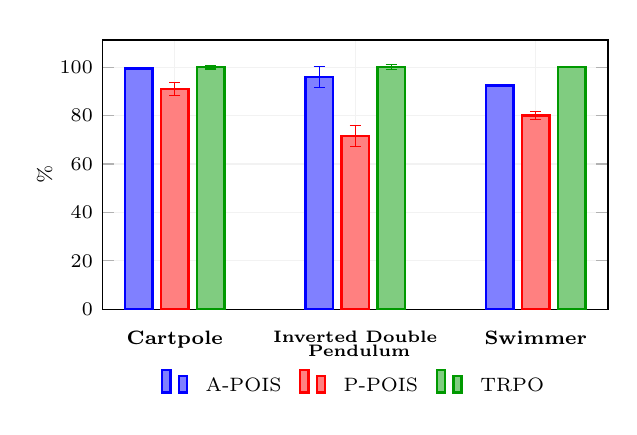
\begin{tikzpicture}
      \begin{axis}[
      grid=both,
grid style={gray!10},
      %legend pos=outer north east,
      %legend style={font=\tiny},
      %axis x line*=bottom,
      %axis y line*=left,
      %ylabel near ticks,
      %xlabel near ticks,     
      every tick/.style={gray!60},
      ylabel={\%},
      height=5cm,
      width=8cm,  
      ylabel style={yshift=-0.15cm},
      %xlabel style={yshift=-0.15cm},
      tick scale binop=\times,
      /pgf/number format/1000 sep={},
      xticklabel style={
        /pgf/number format/fixed,
        /pgf/number format/precision=5
	},
	 every x tick scale label/.style={
             at={(xticklabel* cs:0.92,0.1cm)},
             anchor=near xticklabel
         },
         symbolic x coords={Cartpole, Inverted Double Pendulum, Swimmer},
         xticklabels={\textbf{Cartpole}, $\footnotesize \substack{\text{\textbf{Inverted Double}} \\ \text{\textbf{ Pendulum}}}$, \textbf{Swimmer}},
         ybar=3pt,%ybar=2*\pgflinewidth,
         bar width=10pt,
%      width  = 0.50*\textwidth,
%      height = 8cm,
      major x tick style = transparent,
%      ybar=2*\pgflinewidth,
%      bar width=25pt,
      ymajorgrids = true,
%      
      xtick = data,
      scaled y ticks = false,
      enlarge x limits=0.2,
      ymin=0,
      legend cell align=left,
      legend style={at={(0.5,-0.2)},anchor=north},
      legend style={draw=none, legend columns=-1, column sep=1ex}
  ]
  
  	\addplot[blue, line width=0.3mm, style={fill=blue!50},error bars/.cd, y dir=both, y explicit,error bar style=blue]
           coordinates {
           (Cartpole, 99.44) += (0,0.27) -= (0,0.27)
           (Inverted Double Pendulum,95.95) += (0,4.3) -= (0,4.3)
           (Swimmer,92.4) += (0,0.57) -= (0,0.57)};
           
      \addplot[red, line width=0.3mm, style={fill=red!50},error bars/.cd, y dir=both, y explicit,error bar style=red]
          coordinates {
          (Cartpole, 90.94) += (0,2.8) -= (0,2.8)
          (Inverted Double Pendulum,71.6) += (0,4.29) -= (0,4.29)
          (Swimmer,80) += (0,1.7) -= (0,1.7)};

       \addplot[greencol, line width=0.3mm, style={fill=greencol!50},error bars/.cd, y dir=both, y explicit,error bar style={greencol}]
           coordinates {
           (Cartpole,100) += (0,0.77) -= (0,0.77)
           (Inverted Double Pendulum,100) += (0,1.1) -= (0,1.1)
           (Swimmer,100) += (0,0.21) -= (0,0.21)};

      \legend{A-POIS, P-POIS, TRPO}
  \end{axis}
  \end{tikzpicture}
  \end{document}